
%% Adapted from GaTech CS 7545 Machine Learning Theory given by Prof. Jacob Abernathy Fall 2018. Original latex file: https://github.com/mltheory/CS7545/blob/master/scribe/CS7545scribe_template.tex 



%%%%%PLEASE CONSIDER CORRECTIONS AT PLACES INDICATED%%%%%%%%
\documentclass{article}
%%%%%Packages Used, add more if necessary%%%%
\usepackage{amsmath,amsfonts,amssymb,graphicx,fullpage, float}
\setlength{\topmargin}{-0.6 in}
\setlength{\textheight}{8.5 in}
\setlength{\headsep}{0.75 in}
\usepackage{mdframed}
\usepackage{multicol}
\usepackage{microtype}
\usepackage{hyperref}


%%%%% NO NEED TO EDIT THIS PREAMBLE %%%%%%%%
%%% PREAMBLE %%%
\newcounter{lecnum}
\renewcommand{\thepage}{\thelecnum-\arabic{page}}
\renewcommand{\thesection}{\thelecnum.\arabic{section}}
\renewcommand{\theequation}{\thelecnum.\arabic{equation}}
\renewcommand{\thefigure}{\thelecnum.\arabic{figure}}
\renewcommand{\thetable}{\thelecnum.\arabic{table}}
\newcommand{\lecture}[4]{
   \pagestyle{myheadings}
   \thispagestyle{plain}
   \newpage
   \setcounter{lecnum}{#1}
   \setcounter{page}{1}
   \noindent
   \begin{center}
   \framebox{
      \vbox{\vspace{2mm}
      
      \hbox to 6.28in { 
      {\bf ECE 4252/6252 (FunML) Fundamentals of Machine Learning \hfill 2021--2028} }
      
      \vspace{2mm}
      \hbox to 6.28in { 
      {Courses developed by Professor Ghassan AlRegib 
      (\href{https://alregib.ece.gatech.edu/}{alregib.ece.gatech.edu}) 
      \hfill For inquiries: \href{mailto:alregib@gatech.edu}{alregib@gatech.edu}} }
      
      \vspace{3mm}
      \hbox to 6.28in { {\Large \hfill Lecture #1: #2 \hfill} }
      
      \vspace{2mm}
      \hbox to 6.28in { {\it Co-Instructors: #3 \hfill #4} }
      
      \vspace{2mm}}
   }
   \end{center}

   % -------- PEOPLE OUTSIDE BOX --------
   \vspace{2mm}
   \noindent{\bf Contributors:} Dr. Ahmad Mustafa, Dr. Motaz Alfarraj, Dr. Ashraf Alattar, Dr. Chen Zhou

   \vspace{1mm}
   \noindent{\bf Teaching Assistants} with remarkable contributions include: Kuo-Wei Lai, Wuyang Du, Shiva Mahato, Michael Zhou, Ninghan Zhong

   \markboth{Lecture #1: #2}{Lecture #1: #2}

   \vspace{2mm}
\noindent {\bf Disclaimer}: 
{All content of these notes are part of this course at Georgia Tech. Any re-use or distribution is not permitted without pre-approved permission. All these notes belong to, created by, and copyrighted for Ghassan AlRegib and Mohit Prabhushankar, Georgia Tech, 2021--2028.}

\vspace{2mm}
\noindent {\bf License}: 
{These lecture notes are licensed under the 
\href{https://creativecommons.org/licenses/by-nc-sa/4.0/}{Creative Commons Attribution-NonCommercial-ShareAlike 4.0 International License}.}

   \vspace{2mm}
   \noindent {\bf Errata}: 
   {\it Please submit any errata you find using the following form: 
   \href{https://forms.office.com/r/fbg9dMWPgY}{Errata Form for FunML Textbook} 
   or visit: \url{https://forms.office.com/r/fbg9dMWPgY}}

   \vspace*{4mm}
}
\renewcommand{\cite}[1]{[#1]}
\def\beginrefs{\begin{list}
        {[\arabic{equation}]}{\usecounter{equation}
         \setlength{\leftmargin}{2.0truecm}\setlength{\labelsep}{0.4truecm}%
         \setlength{\labelwidth}{1.6truecm}}}
\def\endrefs{\end{list}}
\def\bibentry#1{\item[\hbox{[#1]}]}

\newcommand{\challenge}[2]{\noindent \textbf{(Challenge Problem)} \emph{#1}: #2 }

\newcommand{\exercise}[1]{\noindent \textbf{(Exercise)} #1 }

\newcommand{\fig}[3]{
			\vspace{#2}
			\begin{center}
			Figure \thelecnum.#1:~#3
			\end{center}
	}
%%% END_OF_PREAMBLE %%%


	
%%%%You may add more \newtheorem if necessary%%%%%%
\newtheorem{theorem}{Theorem}[lecnum]
\newtheorem{lemma}[theorem]{Lemma}
\newtheorem{proposition}[theorem]{Proposition}
\newtheorem{claim}[theorem]{Claim}
\newtheorem{corollary}[theorem]{Corollary}
\newtheorem{definition}[theorem]{Definition}
\newenvironment{proof}{{\bf Proof:}}{\hfill\rule{2mm}{2mm}}


\newcommand{\dom}{\mathrm{dom}}
\begin{document}

\lecture{12}{Clustering and Segmentation Performance Metrics}{Ghassan AlRegib and Mohit Prabhushankar}{}

\noindent\textbf{Keywords:} Clustering evaluation, clustering, performance metrics, anomaly detection, image segmentation

\section{Lecture Objectives}

In this lecture, we study how to evaluate clustering and segmentation performance. We introduce \textbf{internal clustering metrics} such as Davies--Bouldin, Dunn, and Silhouette, and \textbf{external metrics} such as Rand Index, Adjusted Rand Index, Mutual Information, and Purity. We also introduce \textbf{image segmentation metrics}, including pixel accuracy, Intersection over Union (IoU), Dice coefficient, and Hausdorff distance.

\section{Clustering Performance Evaluation}

Clustering algorithms such as k-means, GMM, and mean shift produce partitions of data, but evaluating their quality is non-trivial. In this lecture, we introduce metrics that quantify clustering and segmentation performance under different assumptions.

To assess the quality of a clustering algorithm, we use evaluation metrics that quantify how well the resulting clusters represent meaningful structure in the data. Broadly, clustering evaluation can be divided into two categories. \textbf{External evaluation} measures how closely the computed clusters match a known ground truth set of classes. In contrast, \textbf{internal evaluation} assesses the clustering structure using only the data itself, typically by measuring how compact clusters are and how well-separated they are from one another.

An important requirement of clustering evaluation metrics is that they must be \textbf{independent of the absolute label values}. Since cluster labels are arbitrary identifiers, permuting the label values should not change the evaluation score. In other words, clustering metrics must be permutation-invariant.

\subsection{Internal Evaluation}

In internal evaluation, the clustering result is assessed using only the data that was clustered. These metrics are based on the principle that good clusters should exhibit \emph{high similarity within clusters} (compactness) and \emph{low similarity between clusters} (separation). Algorithms that produce tightly grouped clusters that are well separated from one another will typically achieve higher internal evaluation scores.

However, it is important to note that a high internal score does not necessarily imply good performance in downstream applications such as information retrieval. Additionally, internal metrics may be biased toward algorithms that assume the same cluster structure as the metric itself (for example, centroid-based measures favoring centroid-based clustering methods).

The most commonly used internal clustering metrics are described below.

\subsubsection{Davies–Bouldin Index}

The Davies–Bouldin (DB) Index evaluates clustering quality by comparing intra-cluster compactness with inter-cluster separation. It is defined as:

\[
DB = \frac{1}{k}\sum_{r=1}^{k}\max_{r \neq s}\left(\frac{\sigma_r + \sigma_s}{d(m_r,m_s)}\right)
\]

For each cluster $r$, the DB index computes the worst-case ratio between the sum of within-cluster dispersions and the distance between cluster centroids. The terms in the formula are defined as follows:

Cluster $r$ has centroid $m_r$, and $\sigma_r$ denotes the average distance of all samples in cluster $r$ to its centroid:
\[
\sigma_r = \frac{1}{|C_r|} \sum_{x_i \in C_r} d(x_i, m_r).
\]
The quantity $d(m_r,m_s)$ represents the distance between the centroids of clusters $r$ and $s$.

Intuitively, the DB index measures how similar each cluster is to its most similar neighboring cluster. A smaller DB index indicates better clustering performance, as it reflects compact clusters that are well separated from each other. Therefore, when the goal is to compare cluster separation and compactness, algorithms producing clusters with a \textbf{smaller} DB index are preferred \cite{2}. 

\subsubsection{Dunn Index}
The Dunn Index is denoted by the following formula:\[
D = \frac{\displaystyle \min_{1\leq r\leq s\leq k}d(m_r,m_s)}{\displaystyle \max_{1\leq z\leq k}d'(z)}
\]

The main part is the ratio between the \textbf{minimal inter-cluster distance to maximal intra-cluster distance.}\\
Calculation of $d(m_r,m_s)$ is similar to the one in Davis-Bouldin Index, while $d'(z)$ can also be calculated in a variety of ways(e.g. the maximal distance between any pair of element in cluster $z$)\\
The Dunn Index is particularly useful when the goal is to identify well-separated, compact clusters.\\
Algorithms producing clusters with a \textbf{larger} Dunn Index are preferred \cite{3}.

\subsubsection{Silhouette Coefficient}

The \textbf{Silhouette Coefficient} \cite{4} is an internal clustering metric that evaluates how well each data point fits within its assigned cluster compared to neighboring clusters. It captures both \emph{cluster cohesion} (how close a point is to its own cluster) and \emph{cluster separation} (how far it is from the nearest alternative cluster).

The silhouette value for a sample $x_i$ is computed using the following steps:

\begin{enumerate}
    \item Calculate the average \textbf{intra-cluster dissimilarity} $a_i$ between $x_i \in C_r$ and all other samples in its cluster:
    \[
    a_i = \frac{1}{|C_r|-1}\sum_{x_j\in C_r,\, j\neq i} d(x_i,x_j)
    \]
    
    \item Calculate the average \textbf{nearest-cluster dissimilarity} $b_i$, defined as the smallest average distance from $x_i$ to all samples in any other cluster $C_s$:
    \[
    b_i = \min_{s\neq r}\frac{1}{|C_s|}\sum_{x_j \in C_s} d(x_i, x_j)
    \]
    
    \item Compute the silhouette coefficient:
    \[
    s(x_i)=\begin{cases}
            1-\frac{a_i}{b_i} & \text{if } a_i < b_i \\[6pt]
            0 & \text{if } a_i=b_i \\[6pt]
            \frac{b_i}{a_i}-1 & \text{if } a_i > b_i
            \end{cases}
    \]
\end{enumerate}

\begin{figure}[ht]
    \centering
    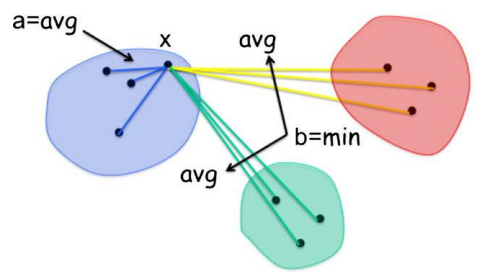
\includegraphics[width=0.4\linewidth]{img/lecture12/Clustering Performance Evaluation/Silhouette Coefficient.png}
    \caption{Figure 12.6: Demonstration of Silhouette Coefficient}
\end{figure}

The silhouette value lies in the range $-1 \le s(x_i) \le 1$. Values close to $1$ indicate that the sample is well matched to its own cluster and far from neighboring clusters, values near $0$ indicate overlapping clusters, and negative values suggest that the sample may be misclassified or represent an outlier. In general, clustering algorithms that produce \textbf{larger average silhouette coefficients} are preferred.

From the silhouette values, we can also construct a \textbf{Cluster Silhouette Plot} by sorting the coefficients in descending order and plotting them vertically for each cluster.

\begin{figure}[ht]
    \centering
    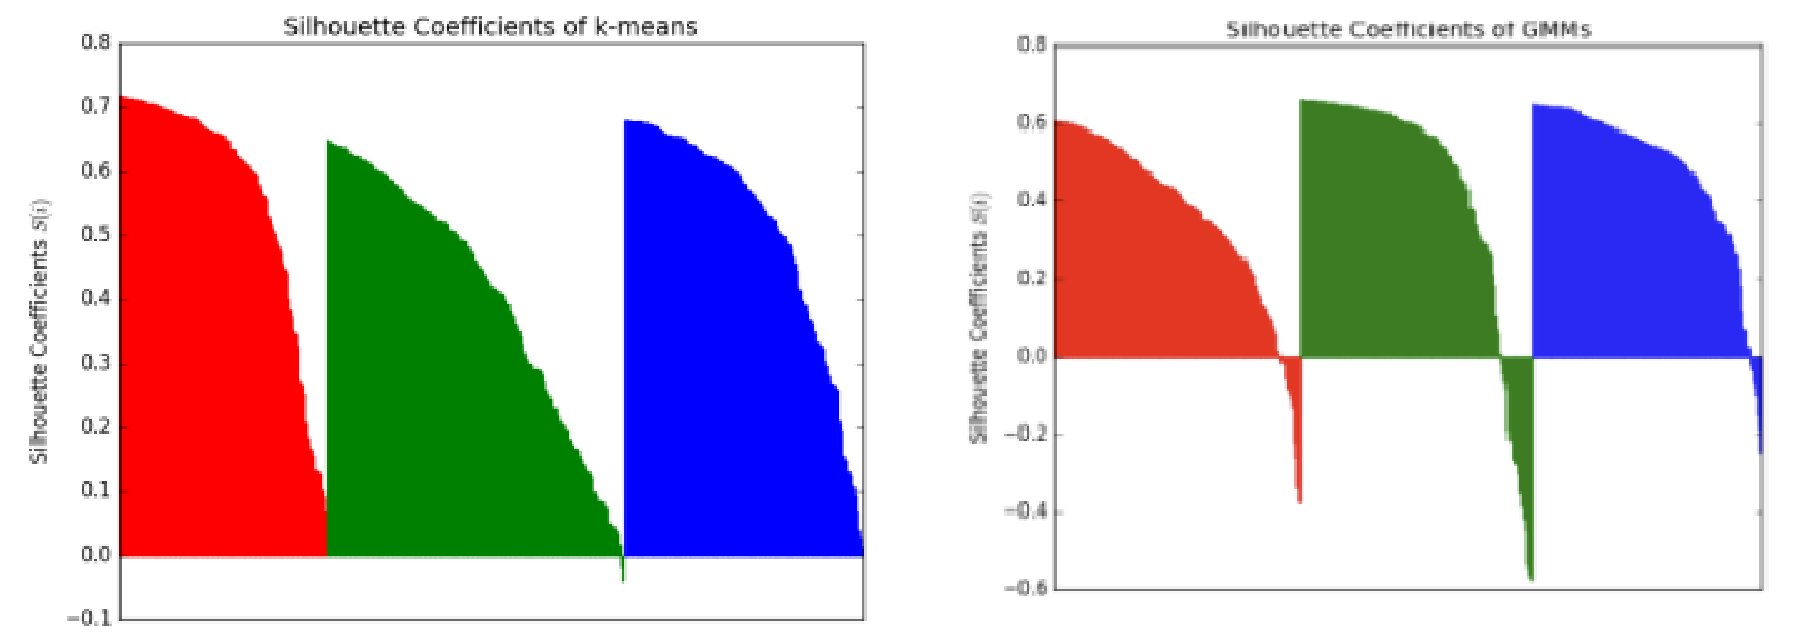
\includegraphics[width=0.8\linewidth]{img/lecture12/Clustering Performance Evaluation/Cluster Silhouette Plot.png}
    \caption{Figure 12.7: Cluster Silhouette Plot of k-means and GMMs}
\end{figure}

The silhouette plot provides a visual summary of clustering quality. Negative coefficients typically correspond to outliers or poorly assigned samples. The thickness of each silhouette region reflects the size of the corresponding cluster, while the mean silhouette coefficient provides a single measure of overall clustering performance. This visualization is therefore useful for assessing and comparing clustering results across different methods. \\

\subsection{External Evaluations}

In \textbf{external evaluation}, clustering performance is assessed using information that was \emph{not} used during the clustering process, such as known class labels or established benchmark datasets. These reference datasets are commonly referred to as the \textbf{gold standard} or \textbf{ground truth}, and they are typically created and validated by human experts. External metrics therefore measure how closely the computed clustering agrees with a known, correct partition of the data.

Throughout this section, we assume the following:
\begin{itemize}
    \item There exists a ground-truth clustering $R = \{R_1, \ldots, R_u\}$ consisting of $u$ clusters.
    \item There exists a computed clustering $Q = \{Q_1, \ldots, Q_v\}$ consisting of $v$ clusters.
\end{itemize}

\subsubsection{Rand Index}
The calculation of Rand Index requires measurement of the following 4 number of pairs:
\begin{enumerate}
    \item $a$: in the same class for both $R$ and $Q$
    \item $b$: in the same class for $R$, but different for $Q$
    \item $c$: in the same class for $Q$, but different for $R$
    \item $d$: in the different class for both $R$ and $Q$
\end{enumerate}
\vspace{30pt}
\begin{figure}[H]
    \centering
    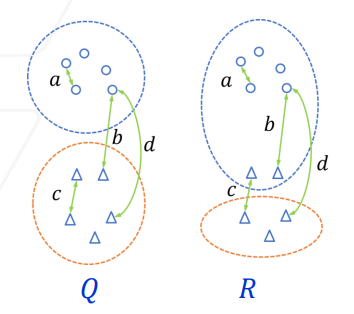
\includegraphics[width=0.4\linewidth]{img/lecture12/Clustering Performance Evaluation/Rand Index.png}
    \caption{Figure 12.8: Rand Index Parameters Demonstration}
\end{figure}
With the four measurements, Rand Index can be denoted as:\[
RI(R,Q)=\frac{a+d}{a+b+c+d}
\]
Rand index can be used to evaluate generated clustering against a ground truth clustering.\\
Algorithms producing clusters with a \textbf{larger} Rand Index are preferred \cite{5}.

\subsubsection{Adjusted Rand Index (ARI)}

When ground-truth labels are available, clustering results can be evaluated using 
external metrics. One widely used metric is the \textbf{Adjusted Rand Index (ARI)}, 
which measures agreement between two partitions while correcting for chance.

The original Rand Index can vary significantly for random clusterings. 
The Adjusted Rand Index addresses this by modeling the random case using a 
generalized hypergeometric distribution \cite{6}. Consequently, the ARI has a maximum value 
of 1, an expected value of 0 for random cluster assignments, and remains meaningful 
even when the compared partitions contain different numbers of clusters.

Assume the dataset contains $N$ samples. Using ground-truth clusters $R$ and computed 
clusters $Q$, we define a \textbf{contingency table} $[n_{ij}]$ where:

\begin{itemize}
    \item $n_{ij}=|R_i \cap Q_j|$
    \item $n_{i,}=\sum_j n_{ij}$ and $n_{,j}=\sum_i n_{ij}$
\end{itemize}

From this table we compute the pair-count quantities of the Rand Index:
\begin{itemize}
    \item $a=\displaystyle\sum_{i,j}\binom{n_{ij}}{2}$
    \item $b=\displaystyle\sum_i\binom{n_{i,}}{2}-a$
    \item $c=\displaystyle\sum_j\binom{n_{,j}}{2}-a$
    \item $d=\displaystyle\binom{N}{2}-a-b-c$
\end{itemize}

The Adjusted Rand Index is then given by:
\[
ARI=\frac{\sum_{i,j}\binom{n_{ij}}{2}-\left[\sum_i\binom{n_{i,}}{2}\sum_j\binom{n_{,j}}{2}\right]/\binom{N}{2}}
{\frac{1}{2}\left[\sum_i\binom{n_{i,}}{2}+\sum_j\binom{n_{,j}}{2}\right]
-\left[\sum_i\binom{n_{i,}}{2}\sum_j\binom{n_{,j}}{2}\right]/\binom{N}{2}}.
\]

\paragraph{Interpretation.}
The numerator represents how much the clustering agreement exceeds chance, while 
the denominator normalizes the score by the maximum possible agreement. 
As a result, ARI provides a robust measure of clustering similarity.

\subsubsection{Mutual Information}
Mutual Information \cite{7} measures the overlap between computed and ground-truth clusters on basis of information theory. The formula for Mutual information score is given as following:\[
MI(R, Q) = \sum_{i=1}^{|R|} \sum_{j=1}^{|Q|} \frac{|R_i \cap Q_j|}{N} \log \frac{N |R_i \cap Q_j|}{|R_i| |Q_j|}
\]
in which,\\
\begin{itemize}
    \item $|R_i|$ is the number of the samples in cluster $R_i$;
    \item $|Q_j|$ is the number of the samples in cluster $Q_j$.
\end{itemize}
Algorithms producing clusters with \textbf{bigger} Mutual Information score is ideal.

\subsubsection{Cluster Purity}
Purity is the measure of the extent to which clusters contain \textbf{a single class}.\\
Purity is defined as how much the \textbf{ground truth} clustering \textbf{matches} the \textbf{computed clustering}, i.e. for a set of $N$ data points the formula is:\[
\frac{1}{N} \sum_{j=1}^{v} \max_{1 \leq i \leq u} |Q_j \cap R_i|
\]

In simplistic terms, add the number of matches for each most matched computed clusters and divide that by the number of data points - that is the purity score. The closer to 1 the purity score is, the better the computed cluster is.\\
The purity score fails to accuracy measure a clustering algorithm if the data is imbalanced between the ground truth clusters.\\

\subsection{Image Segmentation Metrics}

While the clustering metrics above evaluate general partition quality, image segmentation is often evaluated at the \textbf{pixel level} or the \textbf{boundary level}. This is especially relevant for Homework 4, where the output of clustering is interpreted as a segmentation mask.

\subsubsection{Pixel Accuracy}

The simplest segmentation metric is \textbf{pixel accuracy}, which measures the fraction of pixels that are assigned the correct label:

\[
\text{Pixel Accuracy} = \frac{\text{Number of correctly labeled pixels}}{\text{Total number of pixels}}
\]

Pixel accuracy is easy to interpret and is the main metric used in Homework 4. However, it can be misleading when one class dominates the image. For example, if most pixels belong to the background, a method may obtain high pixel accuracy even if it performs poorly on the foreground region.

\subsubsection{Intersection over Union (IoU)}

A more informative overlap-based metric is \textbf{Intersection over Union (IoU)}, also called the \textbf{Jaccard index} \cite{8}. For a predicted segment $P$ and ground-truth segment $G$:

\[
\text{IoU} = \frac{|P \cap G|}{|P \cup G|}
\]

IoU measures how much the predicted region overlaps with the true region relative to their union. Larger IoU indicates better segmentation quality. When multiple classes are present, it is common to average the IoU across classes, yielding the \textbf{mean IoU (mIoU)}.

\subsubsection{Dice Coefficient}

Another common overlap-based metric is the \textbf{Dice coefficient} \cite{9}, defined as:

\[
\text{Dice} = \frac{2|P \cap G|}{|P| + |G|}
\]

Like IoU, Dice measures region overlap, but it places slightly more emphasis on overlap relative to total predicted and ground-truth area. In many segmentation problems, especially when the foreground region is sparse, Dice is preferred because it is less dominated by the background. In large-scale segmentation benchmarks, Dice is often used as the primary pixel-overlap metric, while Hausdorff distance is used to capture structural deviation \cite{1}.

\subsubsection{Hausdorff Distance}

Overlap-based metrics do not fully capture whether boundaries or thin structures are placed correctly. For this reason, segmentation is also evaluated with distance-based metrics such as the \textbf{Hausdorff distance} \cite{10}. A modified Hausdorff distance can be written as:

\[
HD = \max \left(
\frac{1}{N_P}\sum_{p \in P} \min_{g \in G} d(p,g),
\;
\frac{1}{N_G}\sum_{g \in G} \min_{p \in P} d(p,g)
\right)
\]

where $d(\cdot,\cdot)$ is the Euclidean distance between boundary points, and $N_P$ and $N_G$ are the number of points in the predicted and ground-truth sets, respectively.

Hausdorff distance measures the largest average boundary deviation between the predicted segmentation and the ground truth, and is commonly used to evaluate structural accuracy in segmentation benchmarks \cite{1}. Smaller values are better. It is particularly useful when evaluating thin or structured regions, where even small spatial shifts can matter.

\subsubsection{Why Multiple Metrics Are Needed}

Different segmentation metrics emphasize different notions of quality:

\begin{itemize}
    \item \textbf{Pixel Accuracy}: overall fraction of correctly labeled pixels
    \item \textbf{IoU / mIoU}: overlap quality between predicted and true regions
    \item \textbf{Dice}: overlap quality, especially useful for sparse foregrounds
    \item \textbf{Hausdorff Distance}: boundary and structural alignment
\end{itemize}

No single metric is sufficient in all cases. Recent large-scale benchmarks emphasize that overlap-based metrics such as Dice and distance-based metrics such as Hausdorff can disagree, and that some predictions may look visually more reasonable while receiving worse scores under a different metric \cite{1}. This is one reason segmentation performance is often reported using multiple complementary metrics rather than a single number. 

\subsubsection{Connection to Homework 4}

In Homework 4, segmentation quality is primarily evaluated using \textbf{pixel accuracy}. This is a reasonable starting point because it is simple and directly measures the fraction of correctly labeled pixels. However, more advanced segmentation settings often also report IoU, Dice, and Hausdorff distance to better capture overlap quality and structural correctness.

\subsection{Summary of Clustering Metrics}

\begin{center}
\begin{tabular}{| c | c |}
\hline
\textbf{Metric} & \textbf{What it emphasizes} \\ 
\hline

Davies--Bouldin Index & Cluster compactness vs.\ separation (smaller is better) \\  
\hline

Dunn Index & Dense, well-separated clusters (larger is better) \\
\hline

Silhouette Coefficient & Per-sample separability and cohesion (larger is better) \\
\hline

Rand Index & Agreement with ground truth partition (larger is better) \\
\hline

Mutual Information & Shared information with ground truth labels (larger is better) \\
\hline

Cluster Purity & Dominant-class consistency within clusters (larger is better) \\
\hline

\end{tabular}
\end{center}



\subsection{Summary of Image Segmentation Metrics}

\begin{center}
\begin{tabular}{| c | c |}
\hline
\textbf{Metric} & \textbf{What it emphasizes} \\ 
\hline

Pixel Accuracy & Fraction of correctly labeled pixels (larger is better) \\
\hline

IoU / mIoU & Region overlap quality (larger is better) \\
\hline

Dice Coefficient & Overlap quality, especially for sparse foregrounds (larger is better) \\
\hline

Hausdorff Distance & Boundary and structural alignment (smaller is better) \\
\hline

\end{tabular}
\end{center}

% \section{Additional Details}
% This the FYI information and is optional to read about.

% \subsection{Mean Shift Clustering}
% The mean-shift algorithm seeks a mode or \textbf{local maximum} of \textbf{density} of a given distribution, which does \textbf{not require prior} knowledge of the \textbf{number of clusters}.\\
% \\
% In the mean shift algorithm, data points find their mode by \textbf{shifting iteratively towards the mode} until convergence\\
% Note that $K(x_i-x)$ is a kernel function determining the weights of the sample $x_i$ in the window. The algorithm is as follows:
% \begin{enumerate}
%     \item Set a \textbf{window} $W(x)$ around each data point (pre-determined by \textbf{window size/bandwidth})
%     \item Compute the weighted mean of data within the window. $m(x)=\frac{\sum_{x_i\in W(x)} K(x_i-x)x_i}{\sum_{x_i\in W(x)} K(x_i-x)}$
%     \item \textbf{Shift the window to the mean}, $m(x) - x$ is called the mean shift.
%     \item Repeat until $m(x)$ converges, $m(x)$ becomes the mode representing a cluster.
%     \item Merge nearly-identical means, assign each data point to the mean its window
% converges to
% \end{enumerate}
% Computational Complexity
% \begin{enumerate}
%     \item  Needs to shift many windows (a window for each data sample).
%     \item Many computations will be redundant (all samples on the same path are redundant).
% \end{enumerate}
% Mean-Shift Speedup
% \begin{enumerate}
%     \item  Assign all points within radius $r$ of end point to the mode
%     \item Assign all points within radius $r/c$ of the search path to the mode
% \end{enumerate}
% Summary for Mean Shift Clustering
% \begin{itemize}
%     \item Pros
%     \begin{itemize}
%         \item Model-free, does not assume any prior shape (spherical, elliptical, etc.) on data clusters
%         \item Performs clustering using a single parameter (windows size/bandwidth)
%         \begin{itemize}
%             \item Window size has a physical meaning
%         \end{itemize}
%         \item Finds variable number of modes
%         \item Robust to outliers
%     \end{itemize}
%     \item  Cons
%     \begin{itemize}
%         \item Clustering depends on window size
%         \item Windows size/bandwidth selection is non-trivial
%         \item Computationally expensive
%         \item Does not scale well with high dimensional features
%     \end{itemize}
% \end{itemize}
% \subsection{Adjusted Rand Index}
% The problem with Rand index is that the value of it can vary a lot between two random partitions.\\
% To account for that adjusted Rand index assumes the random case as the generalized hyper-geometric distribution. Note that:\\
% \begin{itemize}
%     \item The adjusted Rand index has the maximum value 1, and its \textbf{expected value is 0 in the case of random clusters}
%     \item The adjusted Rand index is recommended for measuring agreement \textbf{even} when the partitions compared \textbf{have different numbers of clusters}
% \end{itemize}
% Use the same notation for ground truth and computed clusters, that there is $N$ elements in the dataset. The \textbf{overlap} between $R$ and $Q$ can be summarized in a \textbf{contingency table} $[n_{ij}]$ where:\\
% \begin{itemize}
%     \item $n_{ij} = |R_i \cap Q_j|$
%     \item $n_{i,}=\sum_{j}^v n_{ij}$ and  $n_{,j}=\sum_{j}^u n_{ij}$
% \end{itemize}
% With this notation we can derive a formula for the values of $a$, $b$, $c$, and $d$ in the original rand index. They are as follows:\\
% \begin{itemize}
%     \item $a=\displaystyle\sum_{i, j}\binom{n_{ij}}{2}$
%     \item $b=\displaystyle\sum_i\binom{n_{i,}}{2} - a$
%     \item $c=\displaystyle\sum_j\binom{n_{,j}}{2} - a$
%     \item $d=\displaystyle\binom{N}{2} - a - b - c$
% \end{itemize}
% The calculation of Adjusted Rand Index is as follows:\\
% \\
% $ARI=\displaystyle\frac{\sum_{i, j}\binom{n_{ij}}{2}-\left[\sum_{i}\binom{n_{i,}}{2}\sum_{j}\binom{n_{,j}}{2}\right]/\binom{N}{2}}{\frac{1}{2}\left[\sum_{i}\binom{n_{i,}}{2}+\sum_{j}\binom{n_{,j}}{2}\right]-\left[\sum_{i}\binom{n_{i,}}{2}\sum_{j}\binom{n_{,j}}{2}\right]/\binom{N}{2}}$\\
% Note:\\
% \begin{itemize}
%     \item $\sum_{i, j}\binom{n_{ij}}{2}$ is the Index
%     \item $\left[\sum_{i}\binom{n_{i,}}{2}\sum_{j}\binom{n_{,j}}{2}\right]/\binom{N}{2}$ is the Max Index
%     \item $\frac{1}{2}\left[\sum_{i}\binom{n_{i,}}{2}+\sum_{j}\binom{n_{,j}}{2}\right]$ is the Expected Index
% \end{itemize}

% \subsection{Image Segmentation}
% The goal of image segmentation is to separate an image into coherent regions. Clustering algorithms can process feature vectors as samples and group them into coherent cluster regions. Those coherent regions can be:
% \begin{itemize}
%     \item Spatial proximity
%     \item Similar color
%     \item Similar texture
% \end{itemize}
% There are a number of potential objectives that can be associated with image segmentation. For a quick survey of different tasks of interest in computer vision, see \href{https://nirmalamurali.medium.com/image-classification-vs-semantic-segmentation-vs-instance-segmentation-625c33a08d50}{here}. Image segmentation in clustering can formulated as:
% \begin{itemize}
%     \item Each pixel is represented by a feature vector $x_i\in\mathbb{R}^{3}$ containing its color channels (RGB).
%     \item Each pixel is represented by a feature vector that use color spaces such as $L^*$ ( luminosity), $a^*$ (red-green), and $b^*$ (blue-yellow).
% \end{itemize}
% Because the color spaces in an image are not equally separable, clustering performance depends on the color space used. In general, given an image we can engineer a set of features (e.g. choosing an appropriate color space) that will best help the model we are using to differentiate between the segments of interest.

% \section{Extensions and Applications of Clustering}

% The clustering methods discussed so far form the core toolkit for unsupervised learning. 
% In this section, we introduce several important extensions, evaluation measures, and 
% applications that build on these ideas.

% \subsection{Mean Shift Clustering}

% The \textbf{Mean Shift} algorithm is a non-parametric clustering method that seeks 
% \textbf{modes (local maxima) of a data density function}. Unlike k-means or GMMs, 
% mean shift does \textbf{not require prior knowledge of the number of clusters}. 
% Instead, clusters naturally emerge as groups of points that converge to the same 
% density mode.

% Intuitively, each data point iteratively moves toward regions of higher density. 
% This is achieved by repeatedly shifting a local window toward the weighted mean of 
% the data within that window. The kernel function $K(x_i - x)$ determines how strongly 
% each neighboring sample influences the update.

% The algorithm proceeds as follows:

% \begin{enumerate}
%     \item Place a \textbf{window} $W(x)$ around each data point, determined by a 
%     user-defined \textbf{bandwidth} (window size).

%     \item Compute the weighted mean of the samples inside the window:
%     \[
%     m(x)=\frac{\sum_{x_i\in W(x)} K(x_i-x)x_i}{\sum_{x_i\in W(x)} K(x_i-x)}.
%     \]

%     \item \textbf{Shift the window} toward the mean. The vector $m(x)-x$ is called 
%     the \textbf{mean shift}.

%     \item Repeat until convergence. The final location $m(x)$ corresponds to a 
%     density mode representing a cluster.

%     \item Merge nearby modes and assign each data point to the mode its window 
%     converges to.
% \end{enumerate}

% \paragraph{Computational considerations.}
% Mean shift can be computationally expensive because a window is shifted for each 
% data sample and many trajectories overlap, leading to redundant computations.

% \paragraph{Common speedups.}
% \begin{enumerate}
%     \item Assign all points within radius $r$ of a converged mode directly to that mode.
%     \item Assign points within radius $r/c$ of the search trajectory to the same mode.
% \end{enumerate}

% \paragraph{Advantages and limitations.}
% Mean shift is appealing because it is \emph{model-free} and makes no assumptions about 
% cluster shape. It uses a single parameter (the bandwidth), which has a clear physical 
% interpretation as the neighborhood size. The method can automatically discover the 
% number of clusters and is generally robust to outliers. 

% However, the quality of the clustering depends heavily on the choice of bandwidth, 
% which can be difficult to tune. The algorithm is also computationally expensive and 
% does not scale well to high-dimensional data.

% \subsection{Application: Image Segmentation}

% An important application of clustering is \textbf{image segmentation}, where the 
% goal is to divide an image into coherent regions. Clustering algorithms treat 
% pixel feature vectors as samples and group them into meaningful regions based on 
% spatial proximity, color similarity, and texture similarity.

% Each pixel can be represented by feature vectors such as RGB color values 
% $x_i \in \mathbb{R}^3$, or by perceptual color spaces such as $L^*$ (luminance), 
% $a^*$ (red–green), and $b^*$ (blue–yellow). Because different color spaces 
% separate visual information differently, clustering performance depends strongly 
% on the chosen feature representation.

% In practice, feature engineering—such as selecting an appropriate color space—plays 
% a key role in producing meaningful segmentation results.

\section{Q\&A Section}
The following table shows the clustering results from two different methods on five samples, along with the ground truth (GT) cluster assignments.

\begin{table}[H]
    \centering
    \begin{tabular}{|c|c|c|c|c|}
        \hline
        Sample & Features & GT Cluster & Method 1 & Method 2 \\ \hline
        1 & [0,1]      & 1          & 1        & 1        \\ \hline
        2 & [1,1]      & 1          & 1        & 2        \\ \hline
        3 & [3,1]      & 2          & 2        & 2        \\ \hline
        4 & [5,1]      & 2          & 3        & 3        \\ \hline
        5 & [6,1]      & 3          & 3        & 3        \\ \hline
    \end{tabular}
    \caption{Clustering outputs of two methods along with ground truth values.}
\end{table}

\begin{enumerate}
    \item \textbf{Question:} \newline
    What is the \textbf{Rand Index (RI)} for each method, calculated across all five samples?
    \newline \newline
    \textbf{Options:}
    \begin{enumerate}
        \item Method 1: 0.80, Method 2: 0.60
        \item Method 1: 0.60, Method 2: 0.85
        \item Method 1: 0.75, Method 2: 0.90
        \item Method 1: 0.80, Method 2: 0.95
    \end{enumerate}
    
    \textbf{Solution:} \newline
    The Rand Index (RI) is calculated as the ratio of the number of agreements between the two clusterings (both in-cluster and out-of-cluster pairs) to the total number of possible pairs. We first need to examine each pair of samples and compare their cluster assignments in both the ground truth and the clustering methods.\\ \\
    For Method 1: 
    \begin{table}[H]
        \centering
        \begin{tabular}{|c|c|c|}
            \hline
            Pairs of Samples & Ground Truth Clusters (GT) & Method 1 Clusters \\ \hline
            (S1, S2) & (C1, C1) & (C1, C1) \\ \hline
            (S1, S3) & (C1, C2) & (C1, C2) \\ \hline
            (S1, S4) & (C1, C2) & (C1, C3) \\ \hline
            (S1, S5) & (C1, C3) & (C1, C3) \\ \hline
            (S2, S3) & (C1, C2) & (C1, C2) \\ \hline
            (S2, S4) & (C1, C2) & (C1, C3) \\ \hline
            (S2, S5) & (C1, C3) & (C1, C3) \\ \hline
            (S3, S4) & (C2, C2) & (C2, C3) \\ \hline
            (S3, S5) & (C2, C3) & (C2, C3) \\ \hline
            (S4, S5) & (C2, C3) & (C3, C3) \\ \hline
        \end{tabular}
        \caption{Cluster Assignments for Ground Truth and Method 1}
    \end{table}
    
    From the table, we can count:
    \begin{itemize}
        \item $a = 1$ (pair (S1, S2) where both GT and Method 1 agree that the clusters are in the same cluster).
        \item $b = 1$ (pair (S3, S4) where GT says same cluster but Method 1 says different).
        \item $c = 1$ (pair (S4, S5) where Method 1 says same cluster but GT says different).
        \item $d = 7$ (remaining pairs where both GT and Method 1 agree that the samples are in different clusters).
    \end{itemize}
    
    Thus, the Rand Index for Method 1 is:
    \[
    \text{Rand Index for Method 1} = \frac{a + d}{a + b + c + d} = \frac{1+7}{1+1+1+7} = 0.80
    \]
    
    For Method 2:
    \begin{table}[H]
        \centering
        \begin{tabular}{|c|c|c|}
            \hline
            Pairs of Samples & Ground Truth Clusters (GT) & Method 2 Clusters \\ \hline
            (S1, S2) & (C1, C1) & (C1, C2) \\ \hline
            (S1, S3) & (C1, C2) & (C1, C2) \\ \hline
            (S1, S4) & (C1, C2) & (C1, C3) \\ \hline
            (S1, S5) & (C1, C3) & (C1, C3) \\ \hline
            (S2, S3) & (C1, C2) & (C2, C2) \\ \hline
            (S2, S4) & (C1, C2) & (C2, C3) \\ \hline
            (S2, S5) & (C1, C3) & (C2, C3) \\ \hline
            (S3, S4) & (C2, C2) & (C2, C3) \\ \hline
            (S3, S5) & (C2, C3) & (C2, C3) \\ \hline
            (S4, S5) & (C2, C3) & (C3, C3) \\ \hline
        \end{tabular}
        \caption{Cluster Assignments for Ground Truth and Method 2}
    \end{table}
    
    From the table, we can count:
    \begin{itemize}
        \item $a = 0$ (no pairs where both GT and Method 1 agree that the clusters are in the same cluster).
        \item $b = 2$ (pairs (S1, S2) and (S3, S4) where GT says same cluster but Method 1 says different).
        \item $c = 2$ (pairs (S2, S3) and (S4, S5) where Method 1 says same cluster but GT says different).
        \item $d = 6$ (remaining pairs where both GT and Method 1 agree that the samples are in different clusters).
    \end{itemize}
    
    Thus, the Rand Index for Method 2 is:
    \[
    \text{Rand Index for Method 2} = \frac{a + d}{a + b + c + d} = \frac{0 + 6}{0+2+2+6} = 0.60
    \]
    
    Hence, the correct answer is \textbf{(a) Method 1: 0.80, Method 2: 0.60}.
    

    \item \textbf{Question 2:} \newline
Compute the Silhouette Score for each sample based on the clusters in Method 1. 
    
\textbf{Solution:} \newline
We use Euclidean distance on the feature vectors. In Method 1 the clusters are:
\[
C_1=\{S1,S2\}, \quad C_2=\{S3\}, \quad C_3=\{S4,S5\}.
\]
Recall:
\begin{itemize}
    \item $a_i$ = average distance to points in the same cluster
    \item $b_i$ = minimum average distance to points in another cluster
    \item $s(x_i)=\frac{b_i-a_i}{\max(a_i,b_i)}$
\end{itemize}
By convention, if a point is the \textbf{only sample in its cluster}, its silhouette value is set to $0$.

\vspace{5pt}
\textbf{Example: Sample 1}

\begin{itemize}
    \item Sample 1 is in Cluster 1 with Sample 2.
    \item Internal dissimilarity:
    \[
    a_1 = d(S1,S2) = \sqrt{(1-0)^2+(1-1)^2}=1
    \]
    \item Distance to Cluster 2:
    \[
    d(S1,S3)=\sqrt{(3-0)^2}=3
    \]
    \item Average distance to Cluster 3:
    \[
    \frac{d(S1,S4)+d(S1,S5)}{2}=\frac{5+6}{2}=5.5
    \]
    Therefore $b_1=\min(3,5.5)=3$.
    \[
    s(x_1)=\frac{3-1}{\max(1,3)}=\frac{2}{3}\approx0.67
    \]
\end{itemize}

Using the same procedure for all samples:

\begin{table}[H]
    \centering
    \begin{tabular}{|c|c|c|c|c|}
        \hline
        Sample & Cluster (Method 1) & $a_i$ & $b_i$ & Silhouette Score \\ \hline
        1 & 1 & 1.00 & 3.00 & 0.67 \\ \hline
        2 & 1 & 1.00 & 2.00 & 0.50 \\ \hline
        3 & 2 & 0.00 & 2.50 & 0.00 \\ \hline
        4 & 3 & 1.00 & 2.00 & 0.50 \\ \hline
        5 & 3 & 1.00 & 3.00 & 0.67 \\ \hline
    \end{tabular}
\end{table}

Hence, the silhouette scores for all samples are shown above.

    \item \textbf{Question 3:} \newline
    Compute the Cluster Purity for both Method 1 and Method 2 based on the ground truth clusters.
    
    \textbf{Solution:} \newline
    For Method 1:
    \begin{itemize}
        \item Cluster 1 (Method 1) has 2 samples, both from GT Cluster 1.
        \item Cluster 2 (Method 1) has 1 sample, which belongs to GT Cluster 2.
        \item Cluster 3 (Method 1) has 2 samples, one from GT Cluster 2 and one from GT Cluster 3.
    \end{itemize}
    
    Purity (Method 1):
    \[
    \text{Purity} = \frac{1}{5} (2 + 1 + 1) = 0.8
    \]
    
    For Method 2:
    \begin{itemize}
        \item Cluster 1 (Method 2) has 1 sample, from Ground Truth Cluster 1.
        \item Cluster 2 (Method 2) has 2 samples, one from Ground Truth Cluster 1 and one from Ground Truth Cluster 2.
        \item Cluster 3 (Method 2) has 2 samples, one from Ground Truth Cluster 2 and one from Ground Truth Cluster 3.
    \end{itemize}
    
    Purity (Method 2):
    \[
    \text{Purity} = \frac{1}{5} (1 + 1 + 1) = 0.60
    \]
    
    Thus, Method 1 has a purity score of 0.80, while Method 2 has a purity score of 0.60.
    

    \item \textbf{Question:} \newline
    Which of the three metrics (Rand Index, Silhouette Coefficient, Purity) would be \textbf{more appropriate} for a dataset where the number of ground truth clusters is unknown, and why?
    \newline \newline
    \textbf{Options:}
    \begin{enumerate}
        \item Rand Index, since it compares to a ground truth.
        \item Silhouette Coefficient, since it measures separation between clusters.
        \item Purity, since it indicates correctness of clustering assignment.
        \item None, because no metric is sufficient when ground truth is unknown.
    \end{enumerate}
    
    \textbf{Solution:} \newline
    The \textbf{Silhouette Coefficient} is more appropriate in cases where the number of ground truth clusters is unknown because it evaluates the quality of the clustering based on how well-separated and compact the clusters are, without needing ground truth labels.

    The correct answer is \textbf{(b) Silhouette Coefficient}.
\end{enumerate}


\section{References}

\beginrefs

\bibentry{1} Quesada, J., Zhou, C., Chowdhury, P., Alotaibi, M., Mustafa, A., Kumakov, Y., Prabhushankar, M., \& AlRegib, G. (2026). \textit{A Large-scale Benchmark on Geological Fault Delineation Models: Domain Shift, Training Dynamics, Generalizability, Evaluation and Inferential Behavior}. arXiv:2505.08585.

\bibentry{2} Davies, D. L., \& Bouldin, D. W. (1979). \textit{A Cluster Separation Measure}. IEEE Transactions on Pattern Analysis and Machine Intelligence.

\bibentry{3} Dunn, J. C. (1974). \textit{Well-separated clusters and optimal fuzzy partitions}. Journal of Cybernetics.

\bibentry{4} Rousseeuw, P. J. (1987). \textit{Silhouettes: A graphical aid to the interpretation and validation of cluster analysis}. Journal of Computational and Applied Mathematics.

\bibentry{5} Rand, W. M. (1971). \textit{Objective criteria for the evaluation of clustering methods}. Journal of the American Statistical Association.

\bibentry{6} Hubert, L., \& Arabie, P. (1985). \textit{Comparing partitions}. Journal of Classification.

\bibentry{7} Strehl, A., \& Ghosh, J. (2002). \textit{Cluster ensembles—a knowledge reuse framework for combining multiple partitions}. Journal of Machine Learning Research.

\bibentry{8} Jaccard, P. (1912). \textit{The distribution of the flora in the alpine zone}. New Phytologist.

\bibentry{9} Dice, L. R. (1945). \textit{Measures of the amount of ecologic association between species}. Ecology.

\bibentry{10} Huttenlocher, D. P., Klanderman, G. A., \& Rucklidge, W. J. (1993). \textit{Comparing images using the Hausdorff distance}. IEEE Transactions on Pattern Analysis and Machine Intelligence.

\endrefs

\end{document}